\documentclass[11pt]{article}
\usepackage{amssymb,amsmath}
\usepackage{dsfont}
\usepackage{times}
\usepackage[left=1in, right=1in, top=1in, bottom=0.5in, includefoot]{geometry}
\setlength\parindent{0.25in}
\setlength\parskip{1mm}

% This package is for including our graph
\usepackage{graphicx}

\title{CMSC601 Research Proposal\\Clustering Metadata for Improved Querying}
\author{Patrick Trinkle\\
Dept. of Computer Science and Electrical Engineering,\\
University of Maryland Baltimore County,\\
Baltimore, MD, 21250\\
\texttt{tri1@umbc.edu}}
\date{May 1st, 2010}

\begin{document}

\maketitle

\section{Introduction}

Typically the goal of an information retrieval system is to aid in locating information, or finding a specific piece of information in a haystack of documents.
Preferably an indexed haystack.
The goal of the proposed information retrieval system is slightly different.
This system's primary goal is to facilitate the discovery of new information.
Effectively, a user who queries the system may find other documents in the corpus that didn't match the criteria of the query, but are related to those documents.
Automatically finding collaborative or buried related information can increase the querier or investigator's knowledge.
There is a limitation however, that the system only applies to a set of corpora that meet specific criteria.

The corpus contains reports such as police reports, travel advisories, business reports, or news reports.
These reports contain metadata, which includes references to other objects in the corpus.
The references can include pointers to other reports, pointers to maps, and any other object that shares information.
Reports also have source information, including the author, possibly a time-stamp, and distribution information.
The general idea is that many documents that are about a specific location or region can include a reference to a map of the area.
These pieces of information in each report can be considered the document metadata.
This system takes it a step further and includes the features of the document, or the important terms in the report, to also be part of the metadata.

A problem inherit with large data sets is that there is more information buried in the corpus than can be visualized or understood.
A large data set is a data set of non-trivial size, such that it is too large for every user to have an entire copy of the data on their system.
Because there is so much data, finding the information you need is difficult.
Another problem inherit with querying large data sets is that you only find what you specify in the query.
Some systems attempt to address this by expanding user queries automatically with semantic data or a thesaurus, but this only finds documents that use similar terms.
A complex data set may have relational structuring linking certain data together.
An effective method for information retrieval against large data sets is the iterative process of querying and refining.
However, with systems that provide the results in simple lists, the process can be tedious.
Viewing the results of queries in different ways can link different concepts visually and also provide for a more fruitful search experience.
Documents have many attributes and features.
These can be contained as metadata for the document including its categories, its term space, its nearest neighbors, its tags, and any previous cluster views.

A measure of performance for search engines in Information Retrieval are three values: precision, recall, and F measure.
Precision is how many of the documents retrieved by the query were judged relevant.
Recall is how many of the relevant documents we retrieved versus how many there were in the corpus.
F measure is a measurement of success as a ratio of precision and recall.

\section{Previous Work}

Finding information in a large data set is an important problem.
This problem has lead many researchers over the past few decades to work towards addressing it.
The problem is also quite large in that there are many niches within the problem that have been effectively solved, while other parts barely explored.
The problem of navigating, searching, and interacting with data falls under multiple categories including Information Visualization, Information Retrieval, and Machine Learning.
To review past works pertaining to the problem, I queried the ACM Digital Library for papers on the at least the following topics: clustering, metadata clustering, interactive clustering, latent semantic analysis, temporal querying, and visual clustering.
The remainder of this section describes the previous work in the fields upon which I am building my research.

\subsection{Information Retrieval}

Before Deerwester et al in 1990, if a user wanted to find a document, they would enter a term or set of well-structured terms into a query engine.  This would then attempt to do plain-text matching against the documents in the system.
The immediate pitfalls of this search method are the following: words can have multiple meanings, words themselves may not appear in the document but their synonyms may.
It was theorized and later proven that the text of a document provides latent semantics.
This information describes the content of a document and the meaning of the content.
Latent Semantic Analysis is the weighing of terms in a document by the semantics derived from the other words in the same and other documents.
If the following word "bar" appears in a few dozen documents, some may refer to a piece of metal while others may refer to a beverage dispensing establishment.
The word "bar" will appear with related words per its definition in a document.
Therefore if a user queries "bar" and related metal terms, documents about the type of building should not be listed because they are semantically unrelated.
There were other improvements, detailed in \cite{Deerwester90}.
Naturally it should follow that if you provide a term with different semantics that it would be useful to see the documents grouped by their subject.
Research in clustering has attempted to address that and related problems.

\subsection{Clustering}

Clustering in terms of documents is the grouping of individual documents into sets based on some criteria.
The criteria for clustering depends on the goal.
Often the goal is to group documents by subject matter.
This is a classification problem.
Given a set of $n$ documents about $k$ topics.
Which documents fall into which of the $k$ groups.
Certainly this problem applies to any user which wishes to find a document and then find similar documents.
Below I have detailed some of the more popular clustering methods as well as clustering topics and ideas upon which some of my research will be based.

Many clustering models view the documents as vectors in an $n$ dimensional vector space.
Each entry in the vector corresponds to the weight of a feature in the document.
The simplest version of this representation is a vector where each 1 represents the presence of a word in a document, and each 0 as the absence of the term.
This straightforward representation compresses well because it is a very sparse matrix.
However, there are more effective representations.
In these vector space models the documents are clustered together based on their corresponding vectors.
One shortcoming of these models is that the size of the feature space can be rather large.
A feature is an attribute of the document, typically a term or word.
Features can also be just pieces of words, n-grams.
k-NN, or k-Nearest Neighbor clusters the documents into whatever category their k-nearest neighbor documents are in.
This is determined by similarity scores.
Similarity scores are calculated a variety of ways; typically cosine similarity is used.
Another clustering model uses centroids.
A centroid is an average representation of a set of input documents in the vector space.
All documents can be processed and merged with their most immediately similar neighbor until all the documents have been processed and form $k$ centroids.
Varying the value of $k$ can directly effect how well the documents are classified or clustered.
Support Vector Machines cluster by attempting to find the largest plane in hyperspace between the documents.
Documents can also be clustered hierarchically, such that a user can drill down into the clusters to find more specific clusters.  This form of clustering is the hierarchical agglomerative method.
It is effectively a hierarchy of centroids that reduce into sets of centroids at each level.
Machine learning can be used to cluster documents and an early example of this is Naive Bayes.
This approach assumes that the probability of a feature appearing in a document is independent of any other term in the document.
Neural networks are also a method of clustering that aim to address the classification problem.
In this problem, the documents must be categorized or clustered to some set of known categories.
Similarly to other machine learning approaches, a training set is used to prime the system.
Guha et al took a hierarchical clustering and improved it by moving away from using a single-point averaged centroid representation and represent clusters with a series of points.
The improvement lies in the loose-form of the cluster themselves, allowing the documents to group in non-spherical ways \cite{Guha1998}.
This work was only tested against a limited sized-data set, however it might be very useful against a larger data set.
This method may not be as useful if the domain is very disjoint.

\subsubsection{Metadata Clustering}

Current Metadata Clustering work attempts to solve the problems associated with distributed document systems.
Interesting queries can be performed against these collections of research papers.
One of these problems is finding social networks within a community of researchers based on their publications.
It can also be used to attempt to distinguish between different authors with the same name.
To build the metadata there are a few interesting methods for automated extraction.
Han et al evaluated using Support Vector Machines for extracting metadata \cite{Han2003}.
Automatically extracting header features is applicable to the research idea, because the header information is part of the metadata.
However, in many of the datasets against which the system is being proposed, the header data is well structured making the automatic extraction problem easier.

\subsubsection{Relational Clustering}

Relational clustering is clustering documents in a relational database where the clusters are determined by what information links together.
Yin et al \cite{Yin2005} approach the issue of relational clustering with help from the users.
Data sets with relational structures may not have obvious correlations.
These correlations may be easily noticed by human users.
It falls onto the issue of language processing, whereby a computer may not have the semantic information to fully link information.
Because the documents I'm looking to query and cluster are in a relational model, with references to other documents and objects in the database or other databases.
The clustering problem is slightly different.
In Yin et al's work the data is spread into various tables that must all be brought together to answer different queries.
However, these human language queries might be difficult for the system to answer without help from the user.

The proposed system will cluster based on query results from the feature-space.
The objects that are linked together will also go into the clustering process, such that documents that didn't match a query may also appear in the results.
Therefore, the proposed system does not purely use relational clustering.

\subsubsection{Query Result Clustering}

In 1992, Cutting et al invented the idea of Scatter/Gather.
The goal of which is to provide an intuitive and effective system for querying a large data set and have the ability to see relationship between the results.
The approach is the system returns a summary of clusters of the documents the query returned.
Each cluster is done hierarchically allowing the user to change granularity.
The user selects clusters that seem relevant to for the search and then the information is reclustered.
This selection process is the Scatter step and the re-clustering is the Gather step \cite{Cutting92}.
This method of grouping results by topic was proven to be very effective in aiding a user's knowledge of the structure and content of a data set \cite{Pirolli96}.
Part of the approach that I don't like is the hierarchical clustering.
This information may miss relationships between data that isn't hierarchical.

\subsection{Feature Space}

The terms or items you use to compare documents are features.
The complete set of all features within the corpus make up its feature space.
It is often a goal of these systems to reduce the feature space.
This can be accomplished with simple methods, such as examining the document frequency and removing singletons and stop words.
Where stop words are terms that are so frequent they have no distinguishing meaning between the documents.
Other approaches include $\chi^2$ and mutual information.
Mutual information and $\chi^2$ both attempt to determine the connection between each pair of terms in the feature space.
Because there can be terms in the feature space with the same meaning, it may be helpful to identify these to reduce size.
Therefore, merging these similar terms can reduce the set of features without losing quality.
Clustering words can reduce the feature space.
This is effectively what is done via principal component analysis.
Principal component analysis reduces a vector space model of the documents to the most important features.

\subsection{User Interface}

A large problem with querying data that the user wants grouped by topic or some other criteria is how to display this information in a human usable and intuitive form.
An appropriate user interface needs to be developed to support interactive querying and clustering.
There has been some work in this field, either with tree hierarchies and some experimental work in interactive graphs.

Most information retrieval systems reply to user queries with lists of matching documents.
The documents are ordered in the results by their rank.
This traditional view is very useful when searching the web, as well as addressing basic document querying problems.
However, it is inadequate to solve the problem this new system seeks to address.

The Scatter/Gather system used a tree view.
This was a list of trees, where each level of each tree was higher granularity within the cluster.
The ability for the user to click on each tree, to drill-down was very useful.
However, this system is also inappropriate for clusters with no hierarchical structure as well as locating documents that share non-content based metadata.

Alonso et al \cite{Alonso2008} extended Scatter/Gather to support user interactions and adjustments to the clusters.
The prototype they built is effective, but has shortcomings if the data set is absurdly large.
The view is all in a tree, listing clusters.
The clusters are grouped hierarchically, allowing the user to drill-down into a subgroups.
This capability to zoom into a cluster, or increase granularity is quite useful.
This work was important because we may be able to extend Scatter/Gather in a similar way, but more similarly to the following paper by desJardins et al.

DesJardins et al built a prototype user interface wherein information was portrayed as clusters.
This system was defined as Interactive Visual Clustering and makes an attempt to cluster the data to address a user's goals.
The interface makes an update to operate on user interactions with the clusters in two dimensions.
Each of the nodes can be dragged by the user to a different "more appropriate" cluster.
Once a user has moved two nodes, the clustering automatically readjusts \cite{desJardins2007}.
The data is clustered based on its attributes, which is similar to what I'm approaching with my user interface.

\section{Proposed System}

The overarching goal of the system is to facilitate knowledge discovery as well as change how users query very large data sets.
This system will remove the chore of browsing or scrolling through lists of results and replace it with a system which attempts to group documents by relevance as well as non-obvious connections.
The system is comprised of three main components of pieces.
The first is the input processing system, which takes the corpus and builds the initial metadata views.
The system will query against the metadata, because it is smaller and should be a good facsimile of the data.
The second portion is the query clustering system, which clusters query results based on their metadata.
Documents that did not immediately match the query are returned as well if they are linked to documents from the query.
The third piece is the graphical user interface.
The GUI for this system is similar to a 3-dimensional grid, where documents are placed in proximity to each other based on their similarity scores.
Links are displayed in between documents based on links in the metadata, such as referencing the same map or other report.
The users can manipulate the document metadata to improving relevance.
Also, previous cluster views of the documents can be stored in the metadata to speedup future similar queries as well as provide suggestions.
It is not unreasonable to consider that if one user finds something interesting, it may be worth investigation by another user.

As previously mentioned, the corpus is a set of reports, such as: travel repositories, police reports, news reports, intelligence reports, SEC filings, business reports, and stock reports.
The focus of a corpus is related to the user's goals and interests.
However, combining several different types of reports could provide for more information.
Such as combining world news reports with business filings.
Something occurring on another side of the world might be directly impacting a company in an unexpected way.
There is however a caveat that this may create too much noise.
Experiments are necessary to help improve the system and allow bringing in many unrelated smaller corpora that might hold corollary information.
Metadata is defined as information about data.
Typically metadata consists of the author, title, publish date, and some keywords.
This system's metadata may vary but should support at least the following: title, author, date/time, gps coordinates, latent semantic feature space, references to addresses, references to phone numbers, references to maps, as well as references to other reports.
See following figure for an example of how the tables could be arranged to support a metadata view of the corpus.
There are foreign key constraints, such that all entries relate back to at least one report in the system.
In this figure, the author's name is followed by a numeric sequence.
This addition of a numeric sequence allows there to be multiple authors with the same name and different unique id values.
Experiments can help determine which fields are the most and the least useful.
This information can be used to refine the user interface.

\begin{center}
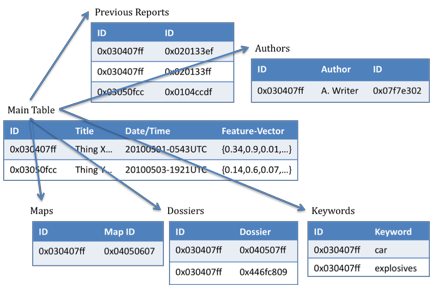
\includegraphics[keepaspectratio=true,scale=0.75]{tableview.png}
\end{center}

Given the system, the following examples are possible:
\begin{enumerate}
\item Searching for information about tribe of interest A.  Query system for reports on tribe A.  Many of the reports have references to maps.  You notice that there are several maps that are also referenced by another cluster of reports.  You examine and find tribe of interest B.  There may be something useful to knowing these two tribes occupy the same region.  Now you have new information that would not have been provided by a different interface.
\item Searching against a database of police reports, you can search for accidents involving pedestrians.  The locations of these may be correlated to an area where there are also lots of recorded incidents of red-light running.  These areas could warrant more police presence.
\item If you enabled temporal data.  The query could run displaying the resulting clusters change over time.  This could provide new insights.  It’s possible that incidents of robbery in certain areas are seasonal.  Albeit, there are probably other ways to ascertain that information.
\item If there are forensic accountants and their data is SEC filings as well as news reports, business reports, and business filings.  They might search for a business and then find other documents in the corpus that share metadata.  The investigators could find another set of business documents connected by address with some documents from another company.  This second company might be doing something illegal, such as hiding money for the first company.
\end{enumerate}

These examples are much more probable with a powerful user interface.

\subsection{Graphical User Interface}

The graphical user interface for the system is very important in helping the user identify new information as well as reduce noise.
Any noise in the system will ideally be clustered away from the query set or possibly scattered as singletons.
The goal of the user interface is to allow the user to glean information by interacting with the view, instead of searching through endless lists.

\begin{center}
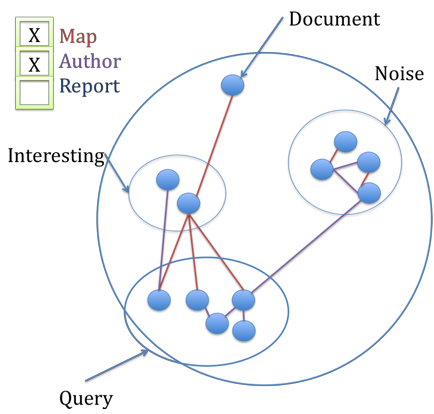
\includegraphics[keepaspectratio=true,scale=0.75]{user_interface.png}
\end{center}

The graphical user interface lists all the metadata features used to link documents (the example only shows three) and these correspond to lines connecting the documents.
To avoid adverse complexity, only certain features will be "on" by default.
If all the features are "on" by default the view would be too crowded to glean information quickly.
This example is only 2-dimensional, whereas users can interact in three Euclidian dimensions.
An advantage to three dimensions, is the clusters are different because they are built from the three most important features instead of the two most important.
This should reduce noise.
Also, because the documents are in three space proximity based on their similarity values, documents that are likely noise are not as intermixed.
Documents that only share links to the query clusters, instead of content similarity are also displayed, to aid in finding correlated data.
The user should be able to zoom into a cluster of documents and even rotate the view.
It is necessary to provide zoom if the clusters are dense.
Rotating the view of the results can aid in gleaning information.
In this demonstration view of the user interface the user entered a query and found other documents that shared a map reference.

\section{Requirements}

To determine the most effective clustering method against the data set, experiments are necessary.
These experiments will attempt to model a subset of the data set under the assumption that the feature space of the domain will not likely increase to the point of invalidation.
Also, the experiments can help determine the scalability of the solution.
If this system is only effective against a very small subset of problem spaces then it may need to be refocused.
To obtain a good sampling of the feature space, the documents chosen to be in the testing set will need to be gathered in a statistically random method.
This may be as simple as giving all documents an index, and using a robust random number generator.
The randomness in document selection is not critical.

The system may also have other currently unknown uses.
Therefore building a prototype for experimentation and then placing the system into different problem spaces may be fruitful.
I estimate that building a prototype may take 6 months, and normalizing a data set may take 2 months.
A prototype for experiments can be ready in 9 months.

\section{Conclusion}

Future work includes building the prototype, determining its limitations and successes, as well as finding other applications for it.
However, the idea is very plausible because I have investigated the usefulness of such a system with investigators.
The general consensus was that reading through lists looking for information was a time sink, and that there was hidden collaborating information in some data sets that takes considerable time to find.

I have recently found that there are people researching similar systems, which try to find situational awareness from clustering of reports.
The system I'm proposing stands on the shoulders of the previous work and combines it to form a more complete solution.
Currently there is no evidence of its ability to improve augmenting user knowledge.  However, this could be collected with a prototype that does not support all of the features.

\bibliographystyle{unsrt}
\bibliography{Proposal}

\end{document}
